\documentclass[aspectratio=169]{beamer}
\usepackage{math214}

\usepackage{babel}
\usepackage{bm}
\usepackage{geometry}

%\usepackage{enumitem}
% Then, after \begin{document}, you can begin your frames/slides

\title{\LARGE 255RC2}
\author{Chengyang Shi, Haoran Shen, Jingfan Tang, Ruizhi Deng}
\date{Summer 2025}

\definecolor{darkblue}{HTML}{6666dd} 
\colortheme{green!30!black}
%\colortheme{orange!85!black}
%\colortheme{darkblue}
%\colortheme{blue!100!black}
%\colortheme{orange!85!white!90!black}
\begin{document}



\maketitle


\begin{frame}
   \frametitle{Contents}
    \tableofcontents     % 生成目录
\end{frame}






    % Example frame
\section{Transpose}
    \begin{frame}{Transpose}
    \begin{block}{Definition}
        $\text{Given } A = (a_{ij}), A^T := (a_{ji})$
    \end{block}
        
        \begin{block}{Proposition}
        Let $A, B$ be matrices, $\lambda \in \mathbb{R}$.
    \begin{enumerate}
        \item $(A+B)^T = A^T + B^T$, $(\lambda A)^T = \lambda A^T $ 
        \item $(AB)^T = B^T A^T$
        \item $(A^T)^T = A$
        \item If $A$ is invertible, so is $A^T$, and $(A^T)^{-1} = (A^{-1})^T$
    \end{enumerate}
    \end{block}
    \end{frame}
    \begin{frame}{Symmetric Matrix}
        \begin{block}{Definition}
            A matrix $A$ is called \textbf{symmetric} if $A = A^T$

            A matrix $A$ is called \textbf{skew-symmetric} if $A^T = -A \iff A + A^T = 0$
        \end{block}
        \begin{block}{Remark}
        \begin{enumerate}
            \item A symmetric or skew-symmetric matrix is necessarily square.
            \item For a skew-symmetric matrix, if $i=j$, then $a_{ij} = 0$
        \end{enumerate}
        \end{block}
        \begin{block}{Example}
            $A = \begin{pmatrix} 1 & -4 & -2 \\ 4 & 1 & 3 \\ 2 & -3 & 2 \end{pmatrix} \text{is not skew-symmetric.}$
        \end{block}
    \end{frame}
\section{Matrix as a Function}
\begin{frame}{Matrix as a Function}
    \begin{block}{Definition}
        An $ n \times m$ Matrix can be interpreted as a function $F: M_{m \times p} \to M_{n \times p}$ 
    \end{block}
    \begin{block}{Property}
        For $M \in M_{n \times m}, A,B \in M_{m \times p}, \alpha , \beta \in \mathbb{R}$ \\
        We have $M(\alpha A + \beta B) = \alpha MA + \beta MB$
    \end{block}
    \begin{block}{Question}
        \begin{enumerate}
            \item Do you know other function with such property?
            \item Why we want such property?
        \end{enumerate}
    \end{block}
\end{frame}
\section{Orthogonal Matrices and Orthonormal Vectors}
    \begin{frame}{Orthogonal Matrix}
        \begin{block}{Definition}
            A matrix $A \in M_n(\mathbb{R})$ is called an orthogonal matrix iff $A^T = A^{-1}$
        \end{block}
        \begin{block}{Properties.} 
        \begin{itemize}
            \item $I_n$ is an orthogonal matrix.
            \item If A and B are orthogonal matrices, then AB is also orthogonal.
            \item If A is an orthogonal matrix, then $A^{-1}$ is also orthogonal matrix.
            \item If A is an orthogonal matrix, then $det(A)= \pm 1$. 
        \end{itemize}
        \end{block}
    \end{frame}
    
\begin{frame}{Orthogonal Matrix}

        \begin{block}{Examples.}
        {$\blacktriangleright$ Rotation Matrix.}
        \par Rotation by $\theta$ in $\mathbb{R}^2$ is given by 
        \begin{equation*}
            \left[ \begin{array}{cc} 
                \cos \theta & -\sin \theta \\ 
                \sin \theta &  \cos \theta \\ 
            \end{array} \right].
        \end{equation*}

        {$\blacktriangleright$ Reflection Matrix.} 
        \par Reflect $(x_1,x_2)$ across $\theta / 2$ in $\mathbb{R}^2$ is given by 
        \begin{equation*}
            \left[ \begin{array}{cc} 
                \cos \theta & \sin \theta \\ 
                \sin \theta & -\cos \theta \\ 
            \end{array} \right]. 
        \end{equation*}
        \end{block}

    \end{frame}
    
    \begin{frame}{Demo}
    You can treat such matrix as a function $Q:$ $\mathbb{R}^2 \to \mathbb{R}^2$
                \begin{figure}
            \centering
            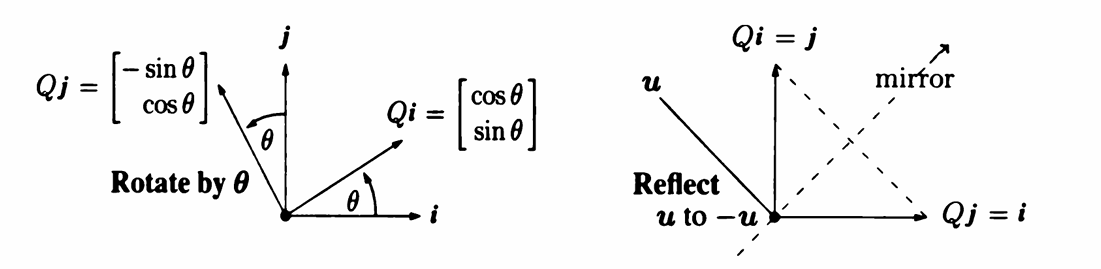
\includegraphics[width=1\linewidth]{demo_rotate&reflect.png}
            \label{fig:enter-label}
        \end{figure}
    \end{frame}
    \begin{frame}{Orthogonal Vectors and Orthonormal Vectors}
        \begin{block}{Definition} 
        Let $\{v_1,\cdots,v_k\} \in \mathbb{R}$ be a subset of $k$ distinct vectors, then $\{v_1,\cdots,v_k\}$ is an \textcolor{red}{orthogonal set of vectors} if $\langle v_i, v_j \rangle = 0$ for all $1 \leq i,j \leq k$, $i \neq j$. 
        
        Also, $\{q_1,\cdots,q_k\}$ is an \textcolor{red}{orthonormal set of vectors} if it is an orthogonal set and all of its vectors are unit vectors (\textit{i.e.}, $\|q_i\| = 1$ for $i \leq i \leq k$).

        \end{block}

        \begin{block}{Remark} 
        Any set containing a single vector is orthogonal; any set containing a single unit vector is orthonormal. 
        \end{block}

        \begin{block}{Example.} $\bar{i},\bar{j},\bar{k} \in \mathbb{R}^3$.
        \end{block}
        
    \end{frame}

    \begin{frame}{Orthogonal Vectors and Orthonormal Vectors}
        \begin{block}{Proposition}
        Given vectors $q_i \in \mathbb{R}^n$, $i = 1,\cdots,m$ such that 
        \begin{equation*}
            \langle q_i , q_j \rangle = q_i^T q_j = \delta_{ij} = \left\{ \begin{array}{ll} 
                1, & i = j, \\ 
                0, & i \neq j, \\ 
            \end{array} \right. 
            (\delta_{ij} : Kronecker)
        \end{equation*}
        then we call the set of vectors $\{q_i\}$ orthonormal, and 
        \begin{equation*}
            Q=\left[\begin{array}{ccc}
                \mid & & \mid \\
                q_{1} & \ldots & q_{m} \\
                \mid & & \mid
                \end{array}\right] \Rightarrow Q^TQ = I_{m}.
        \end{equation*}
        \end{block}

    \end{frame}

    \begin{frame}{Orthogonal Vectors and Orthonormal Vectors}
                \begin{block}{Proof} 
        \begin{equation*}
            \begin{aligned}
                Q^{T} Q &=\left[\begin{array}{ccc}
                - & q_{1}^{T} & - \\
                & \vdots & \\
                - & q_{m}^{T} & -
                \end{array}\right]\left[\begin{array}{ccc}
                \mid & & \mid \\
                q_{1} & \ldots & q_{m} \\
                \mid & & \mid
                \end{array}\right]=\left[\begin{array}{ccc}
                q_{1}^{T} q_{1} & \ldots & q_{1}^{T} q_{m} \\
                \vdots & \ddots & \vdots \\
                q_{m}^{T} q_{1} & \ldots & q_{m}^{T} q_{m}
                \end{array}\right] =I_{m}
                \end{aligned}
        \end{equation*}
        \end{block}
    \end{frame}
    
    \begin{frame}{Orthogonal Matrices and Orthonormal Vectors}
        \begin{block}{Proposition}
            $\text{Let } Q = \begin{bmatrix} | & | & & | \\ \mathbf{q}_1 & \mathbf{q}_2 & \cdots & \mathbf{q}_n \\ | & | & & | \end{bmatrix} \in M_n(\mathbb{R}),$\\
    $\text{where} \{\mathbf{q}_1, \mathbf{q}_2, \dots, \mathbf{q}_n \}$ is a set of orthonormal vectors in $\mathbb{R}^n.$\\
    $\text{Then } Q$ is an orthogonal matrix, $Q^T = Q^{-1}$.\\
    We verify that $QQ^T = I_n$ and $Q^T Q = I_n$.
        \end{block}
    \end{frame}
    

    \begin{frame}{Exercises}

        \par \textcolor{red}{Exercise}
        \par Determine whether the following matrices are orthogonal matrices 
        \begin{equation*}
            \left[ \begin{array}{cc} 
               \frac{\sqrt{3}}{2}& -\frac{1}{2} \\ 
                \frac{1}{2} &  \frac{\sqrt{3}}{2} \\ 
            \end{array} \right].
        \end{equation*}

        \begin{equation*}
            \left[ \begin{array}{cc} 
                1 & 1 \\ 
                1 & -1\\ 
            \end{array} \right]. 
        \end{equation*}
    \end{frame}
\begin{frame}{Orthogonal Matrices and Orthonormal Vectors}
    \begin{block}{Proposition}
The orthogonal matrices are precisely the matrices that preserve the inner product in $\mathbb{R}^n$ \\
i.e., $\forall x,y \in \mathbb{R}^n$, $\langle x,y \rangle = \langle Ax, Ay \rangle$
or $x^T y = (Ax)^T Ay$.
\end{block}

\begin{proof}
If $A$ is orthogonal, i.e., $A^{-1} = A^T$,
then $A^T A = I_n$, so $(Ax)^T (Ay) = x^T A^T A y = x^T I_n y = x^T y$.
\end{proof}
\end{frame}
\begin{frame}{Why we need Orthonormal Matrix?}
    \begin{enumerate}
    \item \textbf{Magnitude of Determinant and Column Norms:}
    \begin{itemize}
        \item $|\det(A)| = 1$.
        \item Column vectors $\bm{q}_i$ have unit norm: $||\bm{q}_i|| = 1$.
        \item \textit{Implication:} The transformation represented by $A$ is a rotation or a reflection.
    \end{itemize}

    \item \textbf{Defining Property and Its Consequences:}
    \begin{itemize}
        \item $A^T A = I_n$ (which means $A^{-1} = A^T$).
        \item The original note mentions this "has very good symmetric properties."
        \item \textit{Implications include:}
        \begin{itemize}
            \item Preservation of inner products (hence, lengths and angles are preserved: $\langle Ax, Ay \rangle = \langle x, y \rangle$).
            \item The inverse $A^{-1}$ is easy to compute (it's just the transpose $A^T$).
        \end{itemize}
    \end{itemize}

    \item \textbf{Applications in Data Processing:}
    \begin{itemize}
        \item Effective in removing redundant information from data
    \end{itemize}
\end{enumerate}
\end{frame}

\section{Kernel and Image}
\begin{frame}{Kernel and Image}
    \begin{block}{Definition}
        \begin{itemize}
    \item Given matrix $A \in M_{m \times n}(\mathbb{R})$. The kernel, or nullspace of $A$, is defined as
    \[
    \operatorname{ker} A = N(A) = \{x \in \mathbb{R}^n \mid Ax = \mathbf{0}\} \subseteq \mathbb{R}^n
    \]
    where $A: \mathbb{R}^n \rightarrow \mathbb{R}^n$.

    \item The image of $A$, or column space, is defined as
    \begin{align*}
    \operatorname{im} A = C(A) &= \{y \in \mathbb{R}^m \mid \exists x \in \mathbb{R}^n, y = Ax\} \\
    &= \{Ax \mid x \in \mathbb{R}^n\}
    \end{align*}
    (The image is a subspace of $\mathbb{R}^m$).
\end{itemize}
    \end{block}
\end{frame}

\begin{frame}{Injectivity}
    \begin{block}{Definition}
        A function $f: A \to B$ is called injective, if \\
        $\forall x_1, x_2 \in A, f(x_1) = f(x_2) \implies x_1 = x_2$ \\
        i.e., $\forall x_1, x_2 \in A, x_1 \neq x_2 \implies f(x_1) \neq f(x_2)$
    \end{block}
    \begin{block}{Proposition}
        Given $A \in M_{m \times n}(\mathbb{R})$, i.e., $A: \mathbb{R}^n \to \mathbb{R}^m$ \\
        then, A is injective $\iff \ker A = N(A) = \{0\}$
    \end{block}
\end{frame}

\begin{frame}{Injectivity}
    \begin{block}{Proof}
        ($\Rightarrow$) Assume A is injective, that is, \\
$\forall x_1, x_2 \in \mathbb{R}^n, Ax_1 = Ax_2 \implies x_1 = x_2$.

Take $v \in \ker A$, i.e., $Av = 0$.
We also know that $A0 = 0$, hence $Av = A0$.
By injectivity of A, $v=0$. Therefore $\ker A = \{0\}$.

($\Leftarrow$) Conversely, suppose $\ker A = \{0\}$.

Take $v_1, v_2 \in \mathbb{R}^n$, s.t. $Av_1 = Av_2$.
We want to show that $v_1 = v_2$.
Indeed, we have $A(v_1 - v_2) = 0$, but $\ker A = \{0\}$,
hence $v_1 - v_2 = 0$. So $v_1 = v_2$.
    \end{block}
\end{frame}

\begin{frame}{Kernel and Image}
    \begin{block}{Proposition}
        Given $A \in M_{m \times n}(\mathbb{R})$ , $\ker(A) = \ker(A^T A)$ 
    \end{block}
    \begin{block}{Proof}
        ($\subseteq$) Take $x \in \ker(A)$, i.e., $Ax=0$.
So $(A^T A)x = A^T(Ax) = A^T 0 = 0$.
So $x \in \ker(A^T A)$.

($\supseteq$) Take $x \in \ker(A^T A)$, i.e., $A^T Ax = 0$.
So $x^T A^T Ax = x^T 0 = 0$.
$(Ax)^T Ax = \|Ax\|^2 = 0$.
$\implies Ax = 0 \implies x \in \ker A$.
($v_1^2 + v_2^2 + \dots + v_n^2 = 0 \implies v_i = 0$)
    \end{block}
\end{frame}

\section{Projection Matrix}
\begin{frame}{Projection Matrix}
    \begin{block}{Definition}
        A matrix $P \in M_n(\mathbb{R})$ is a projection matrix, if $P^2=P$.
        
        It is called an orthogonal projection, if $P=P^T$.
    \end{block}
    \begin{block}{Example}
        For an orthonormal matrix $Q$
        \begin{itemize}
            \item $(QQ^T)^T = (Q^T)^T Q^T = Q Q^T$
            \item $(QQ^T)^2 = (QQ^T)(QQ^T) = Q(Q^T Q)Q^T = Q I_k Q^T = QQ^T$ 
        \end{itemize}
        $Q Q^T: \mathbb{R}^n \to \mathbb{R}^n \text{ is a projection}$
    \end{block}
\end{frame}
\begin{frame}{Orthogonal Projection Matrix}
    \begin{block}{Proposition}
        A projection matrix $P$ is an orthogonal projection if
$$ \ker P \perp \operatorname{im} P $$
i.e., $\forall x \in \ker P$, $\forall y \in \operatorname{im} P$,
$$ \langle x, y \rangle = x^T y = 0 \in \mathbb{R} $$
    \end{block}
    \begin{block}{Exercise}
    Show that $ \ker P \perp \operatorname{im} P $ if $P = P^T$
\end{block}    
\end{frame}
\begin{frame}{Orthogonal Projection Matrix}
\begin{block}{Example}
    $$
 \{q_1, q_2\} = \left\{ 
\begin{pmatrix} 1/\sqrt{2} \\ 1/\sqrt{2} \\ 0 \end{pmatrix}, 
\begin{pmatrix} 1/\sqrt{2} \\ -1/\sqrt{2} \\ 0 \end{pmatrix} 
\right\}
$$

$$
Q = \begin{bmatrix} 
1/\sqrt{2} & 1/\sqrt{2} \\ 
1/\sqrt{2} & -1/\sqrt{2} \\ 
0 & 0 
\end{bmatrix}, \quad 
Q^T = \begin{bmatrix} 
1/\sqrt{2} & 1/\sqrt{2} & 0 \\ 
1/\sqrt{2} & -1/\sqrt{2} & 0 
\end{bmatrix}
$$

$$
QQ^T = \begin{bmatrix} 
1 & 0 & 0 \\ 
0 & 1 & 0 \\ 
0 & 0 & 0 
\end{bmatrix}
\begin{pmatrix} x \\ y \\ z \end{pmatrix}
= 
\begin{pmatrix} x \\ y \\ 0 \end{pmatrix}
$$
\end{block}

\end{frame}


\begin{frame}{Reference}
    \begin{enumerate}
        \item VV255, Lecture Notes 24SU, Runze Cai
        \item VV255 RC2, Jiayue Huang, et al
        \item Introduction to Linear Algebra, Sixth Edition, Gilbert Strang
    \end{enumerate}
\end{frame}

\begin{frame}{\textcolor{green!30!black}{end}}
    \begin{center}
        \LARGE Thank you and Enjoy your Summer Semester!
    \end{center}
\end{frame}
\end{document}